\chapter*{Canceling Orders}\label{ch:canceling}\index{Canceling Orders}
% \section{Introduction}
\newthought{Orders can be canceled} as long as the results have not been verified. The lab can cancel orders using a few different ways. This procedure will guide the trainee through canceling orders using {orv} and {pending inquiry}Orders can be canceled

% \vspace{4\baselineskip}

% \vspace{-4\baselineskip}


\bigskip

\newthought{Required training} before proceeding with this section%
\marginnote{This guide assumes that the user is familiar with these functions}.
\begin{itemize}
   \item Cerner App-Bar
   \item {Pending Inquiry}
   \item Order Result Viewer
   \item Entering Comments
 \end{itemize}


\newthought{When is it possible } to cancel? if the order status in {orv} is listed as {in-lab} it can be canceled. It will be credited by the system automatically. Once any portion of a test has been resulted (e.g. Glucose within a BMPNL) the order status, in {order result viewer}, will change to In Process and it can no longer be canceled.


\bigskip
\bigskip


\begin{minipage}{\textwidth}
\noindent
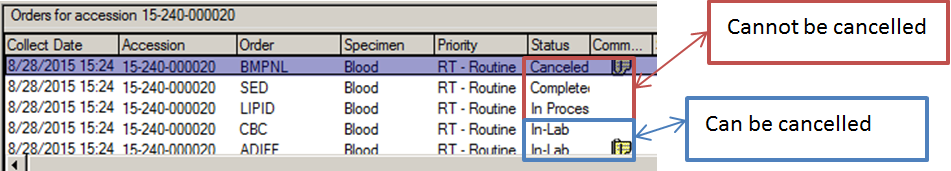
\includegraphics[width=\textwidth]{ORV/graphics/statuses.png}
\end{minipage}
% \vspace{3\baselineskip}
\marginnote[-4\baselineskip]{If the order status is Completed or In Process the rest of the order must be resulted with a freetext result and the test must be credited.}

\cfsection*{}{ORV}{cancel.tex}
\cfsection*{}{PENDING}{cancel.tex}

